\documentclass[a4paper,12pt]{article}

% Language and encoding
\usepackage[utf8]{inputenc}
\usepackage[english]{babel}

% Proper date format
\usepackage[yyyymmdd]{datetime}

% For front page
\usepackage{wallpaper}

% For tables
\usepackage{tabularx,ragged2e,booktabs}

% For margin
\usepackage[margin=3cm]{geometry}

% For math
\usepackage{amsmath,amssymb,amsthm}
\usepackage{xfrac}
\usepackage{mathtools}
\usepackage{bm}

% For href
\usepackage{hyperref}

% Linux Libertine Font
\usepackage[T1]{fontenc}
\usepackage[tt = false]{libertine}

% For quotes
\usepackage{csquotes}

% For figures
\usepackage{graphicx}
\usepackage{caption}

% For figure positioning (allows use of H)
\usepackage{float}

% For references
\usepackage[backend=biber, style=numeric, sorting=none]{biblatex}
\addbibresource{references.bib}

% For paragraph skipping
\usepackage{parskip}

% For appendix
\usepackage[toc,page]{appendix}

% For text coloring
\usepackage{color}

% For enumeration with letters
\usepackage{enumerate}


% Chapter formatting
\titleformat{\chapter} % command
    [display] % shape
    {\bfseries\huge} % format
    {\thechapter} % label
    {0.0pt} % separator
    {} % before-code
    [] % after-code

% Spacing of sections         Left      Before spacing           After spacing      [right] (optional)
\titlespacing*{\chapter}      {0pt}{0pt plus 2pt minus 2pt}{8pt plus 2pt minus 2pt}
\titlespacing*{\section}      {0pt}{8pt plus 2pt minus 2pt}{4pt plus 1pt minus 1pt}
\titlespacing*{\subsection}   {0pt}{8pt plus 2pt minus 2pt}{2pt plus 1pt minus 1pt}
\titlespacing*{\subsubsection}{0pt}{4pt plus 1pt minus 1pt}{2pt plus 1pt minus 1pt}

% Declaring definitions, theorems etc.
\newtheorem*{definition}{Definition}
\newtheorem*{theorem}{Theorem}
\newtheorem*{lemma}{Lemma}
\newtheorem*{claim}{Claim}
\newtheorem{corollary}{Corollary}
\newtheorem{example}{Example}

% -- Commands
% TODO macro
\newcommand{\todo}[1]{{\color{red} TODO: { #1 }}}

% Internal formatting method
\newcommand{\mo}[1]{{\mathopen{} #1 \mathclose{}}}

% Differential d
\newcommand*\diff{\mathop{}\!\mathrm{d}}

% Line segments
\newcommand{\overbar}[1]{\mkern 1.5mu\overline{\mkern-1.5mu#1\mkern-1.5mu}\mkern 1.5mu}

% Vector
\newcommand{\ve}[1]{\mathbf{ #1 }}

% Scaling parentheses
\newcommand{\prts}[1]{\mo{\left( #1 \right)}}

% \DeclarePairedDelimiter{\prts}{\left(}{\right)}

% Scaling curly brackets
\newcommand{\crts}[1]{\mo{\left\{ #1 \right\}}}

% Scaling brackets
\newcommand{\brts}[1]{\mo{\left[ #1 \right]}}

% Expected value
\newcommand{\E}[1]{\mathbb{E}{\mo{\left[ #1 \right]}}}
% Variance
\newcommand{\Var}[1]{\mathrm{Var}{\mo{\left[ #1 \right]}}}

% Floor and ceil
\newcommand{\ceil}[1]{\left\lceil #1 \right\rceil}
\newcommand{\floor}[1]{\left\lfloor #1 \right\rfloor}

% Absolute value
\DeclarePairedDelimiter{\abs}{\lvert}{\rvert}


\DeclareMathOperator{\kullbackliebler}{kl}
\newcommand{\kl}[2]{\kullbackliebler\mo{\left(#1 \parallel #2\right)}}

% Listing color syntax
\definecolor{greybg}{RGB}{246,247,248}
\definecolor{codeblue}{RGB}{15,126,227}
\definecolor{codegreen}{rgb}{0,0.6,0}
\definecolor{codegray}{rgb}{0.5,0.5,0.5}
\definecolor{codepurple}{rgb}{0.58,0,0.82}
\definecolor{backcolour}{rgb}{0.95,0.95,0.92}
\definecolor{redstrings}{rgb}{1,0.6,0.6}
 
\lstdefinestyle{mystyle}{
    backgroundcolor=\color{greybg},   
    commentstyle=\color{codegreen},
    keywordstyle=\color{codeblue},
    numberstyle=\tiny\color{codegray},
    stringstyle=\color{codepurple},
    basicstyle=\footnotesize\ttfamily,
    breakatwhitespace=false,         
    breaklines=true,                 
    captionpos=b,                    
    keepspaces=true,                 
    numbers=left,                    
    numbersep=5pt,
    showspaces=false,                
    showstringspaces=false,
    showtabs=false,                  
    tabsize=2,
}

\lstset{style=mystyle, lineskip=2pt}

\begin{document}

% Title
\title{
    \vspace{6cm}
    \Huge{\textbf{Reproduction and Evaluation of UniRep, a Deep Learning Representation of Protein Sequences}} \\
}

% Author
\author{\Large{Emil Petersen} \\ \href{mailto:empe@di.ku.dk}{\textbf{[empe@di.ku.dk]}} \and \Large{Victor Nordam Suadicani} \\ \href{mailto:nordam@di.ku.dk}{\textbf{[swl460@alumni.ku.dk]}}
}

% Date set automatically
% \date{}

% Background
\ThisCenterWallPaper{1.0}{nat-farve.pdf}
\ThisCenterWallPaper{1.0}{nat-en.pdf}

\AddToShipoutPicture*{\put(100,120){Supervisors: Wouter Krogh Boomsma}}

% Insert title, author and date
\maketitle

% No page numbering please
\thispagestyle{empty}

% Sections start on next page, which is considered page 1
\newpage
\setcounter{page}{1}


% No page numbering please
\thispagestyle{empty}
\tableofcontents
\clearpage
\setcounter{page}{1}

\section{Introduction}

Proteins are essential to many biological industries, including the medicinal industry and the food industry. Due to proteins' importance in these industries, a lot of effort has been made towards developing new proteins which could be useful for biological processes. The field concerned with design and synthesis of such proteins is known as \textit{protein engineering}. There are two main approaches within protein engineering: directed evolution and rational protein design. The former attempts to find new proteins by simulating natural evolution -- we will not concern ourselves with this approach any further. The latter takes a more direct approach to protein engineering; rational design tries to construct an amino acid sequence given a desired 3-dimensional structure. In this work, we are considering a related problem which could be useful to rational protein design, that is, prediction of structure and properties given an amino acid sequence.

Effective usage of machine learning techniques on the domain of protein engineering has long been sought. For many years, protein engineering has suffered from the lack of a holistic understanding of protein structure and function. Recently, advances in deep learning techniques have brought new hope to this endeavor. With advanced techniques from the field of deep representation learning, machine learning systems may be able to learn rich representations of proteins, without a need for manual feature extraction. Such representations could be highly relevant to downstream tasks within protein engineering.

In this report, we examine a recent paper \cite{alley2019unified} (UniRep paper) utilizing deep representation learning on protein sequences. In it, Alley et al. present a novel protein representation learning model. The authors and creators of the UniRep model make promising claims, and give several performance and quantitative tests to support this. In this report, we investigate the methods used to yield the model, and reproduce some of the more prominent results. In addition we seek to clarify the reasoning behind the design choices and any significant trade-offs these choices require. 

Before we discuss the results, we provide some background information. The UniRep model relies on recurrent neural networks and a compressed representation of protein sequences. We will provide some background explanations required to understand the modelling part. There are also several nontrivial performance metrics that will be covered in this report for the sake of understanding. Finally, we will briefly discuss the downstream tasks and what they entail.

The UniRep paper itself is discussed in its own section, providing the article's key contributions, motivation and results.

The remainder of the report presents and discusses the key reproduced results and how they measure in comparison with the UniRep paper results. This includes a critical inspection of some of the claims made and ultimately some suggestions for future work and alternative approaches.

% Outlining the motivation for the research
% Explaining the main contribution of the paper
% Discussion of the key results
% Concluding remarks and opportunities for future research

\clearpage
\section{Background}
\label{section:background}

In this section we first present the main model architectures used in the UniRep article \cite{alley2019unified}. Specifically, the idea and governing principles of Recurrent Neural Networks (RNN) are introduced, giving the necessary knowledge to understand specific variants of RNNs. Then three different RNN models are presented, namely the Long Short-Term Memory (LSTM), the Gated Recurrent Unit (GRU) and the multiplicative LSTM (mLSTM), the latter being the model architecture used in the UniRep article.

We use a series of downstream tasks to measure the performance of our implementation; these tasks are directly chosen based on the learning tasks and surveyed benchmarks by \cite{tape2019}. These require an introduction, which will be given here, under section \ref{section:tape}, as well as what performance metrics are used in these tasks.
% mLSTM:
% https://arxiv.org/pdf/1609.07959.pdf

\subsection{Recurrent Neural Networks}
Recurrent Neural Networks are neural networks used mainly for sequential, temporal data, where inputs usually differ in length. There are several ways to work with sequences: we might wish to predict a label for each single character in the sequence, effectively yielding a sequence output of labels; or we wish to predict a single label for the entire sequence. In any case, modelling structures are needed to support the task and there are many commonly used variants of RNNs.

For some input sequence $\ve{S} = s_1, s_2, \ldots, s_T$ of length $T$ consisting of characters from a pre-specified alphabet, an RNN processes the input one character $s_t$ at a time (with time step $t \leq T$). In the case of protein sequencing, the time step simply refers to the position in the sequence. In this process, the RNN usually maintains an internal context state (also known as a \textit{hidden state}) that retains information from the sequence up to $t$. In most practical settings, the state is not complex enough to keep a one-to-one representation of the sequence observed so far, and thus needs to effectively prioritize what it will retain or not. By a combination of the current input $s_t$ and this context state, the RNN produces an output. For example, this output could be a prediction of the sequence character at time $t + 1$. To do this, the network passes the internal state and input through one or more operations, each with its own parameters.

Viewed as a graph, the RNN is a series of layers (or layered cell structures for more advanced model instances), processing the sequence one character at a time. The parameters of the model is shared across the components of the network, meaning that the parameters are reused at each time step. This enables the model to process sequences of variable length as the model is specified in terms of transitions between characters, rather than on the entire sequence. This has the desirable property that the model is able to generalize to inputs with a previously unseen length. Because parameters are used across different time steps, they are used to learn general rules that work not just at the beginning or end, but across the entire sequence \cite{Goodfellow-et-al-2016}.

In addition, RNN's have the desirable property that the internal state is flexible in terms of learning what context is important and what can be disregarded. However, one disadvantage is that, for simple RNN's, it is difficult to make the model retain important information across long sequences, i.e. the context at some step $t$ will not contain much information from a time step $s \ll t$. To remedy this, more elaborate architectures have been designed that incorporate specific internal cell states to retain context \cite{graves2012supervised}. Specifically, the LSTM and GRU architectures do this, which we discuss in section \ref{section:LSTM} and \ref{section:GRU}. The mLSTM architecture used in the UniRep paper is a variation on the LSTM.

Networks that use the same function iteratively on sequenced inputs are typically represented as a recursive formula. A typical example is
\[ \ve{h}_t = f\prts{\ve{x}_t, \ve{h}_{t - 1}}, \]
where the context state $\ve{h}_t$ at time $t$ is the result of applying a function $f$ to the input character $\ve{x}_t$ at time $t$ and the previous context state $\ve{h}_{t - 1}$. Such representations allow for a simple description that conveys what dependencies there are between inputs, without unrolling the entire recursive structural dependency. Some models might require several such relations to describe it. We will use such representations to formally describe RNNs.

In a single forward pass (one time step) in a typical simple RNN, the following calculations are done:
\begin{align*}
    \ve{a}_t &= \ve{b} + \ve{Wh}_{t - 1} + \ve{Ux}_t\\
    \ve{h}_t &= f_1 \prts{\ve{a}_t}\\
    \ve{o}_t &= \ve{c} + \ve{Vh}_t\\
    \hat{\ve{y}}_t &= f_2 \prts{\ve{o}_t}.
\end{align*}
Here, $\ve{W}$ and $\ve{U}$ are the parameters for the previous hidden state $\ve{h}_{t-1}$ and the current input $\ve{x}_t$ and $\ve{b}$ is the bias. Similarly $\ve{V}$ contains the parameters for the current hidden state $\ve{h}_t$ and $\ve{c}$ is a bias. Finally, $f_1$ and $f_2$ are (activation) functions applied to the intermediate results $\ve{a_t}$ and $\ve{o}_t$ to yield the current hidden state and the prediction $\hat{\ve{y}}_t$. This forward pass assumes an RNN where the previous hidden state is passed as input to the next, but other variations exists.

% During training, a popular choice is to disregard the model prediction when passing the current input and instead feed the model the true character for the ensuing iteration. This procedure is usually called \textit{teacher forcing}, which ensures that the hidden state is based on a true sequence and not (potentially wrong) model predictions.

The backpropagation in RNN's is no different from `ordinary' neural networks; the parameters are updated using a gradient-based optimizer, taking advantage of the network operations being differentiable by design. For each model output prediction, a loss is computed with respect to the true label. The gradient of the loss is calculated using the chain rule, with respect to the parameters of the model. This gradient is then used to update the parameters, effectively lowering the error. This procedure is repeated until the loss is sufficiently low, or a similar termination condition is met. The algorithm is in this case referred to as backpropagation through time (BPTT), as each iteration is dependent on the hidden state of the previous iteration. This dependency makes the backward pass sequential, and so it is computationally expensive for longer sequences as it cannot be easily parallelized. For this reason, a truncated version (TBPTT) is often applied instead, which splits the sequence into a number of smaller sequences and updates weights after each sequence is processed. This has the effect that each pass gives more weight updates, and the backpropagation can thus be computed across longer sequences more effectively. It also has the negative effect that context spanning across splits are lost. TBPTT is used in the UniRep article experiments \cite{alley2019unified}.

\subsubsection{Long Short-Term Memory}
\label{section:LSTM}
The Long Short-Term Memory (LSTM) architecture is an RNN which incorporates additional modelling to make the network more persistent across time. The hidden state in simple RNNs have difficulties retaining a context that ``remembers'' across longer sequences, i.e. long-term dependencies. One problem is that gradient propagation over long sequences tend to produce very small (vanishing) gradients, effectively nullifying any updates done to the parameters. A partial solution is to apply activation functions that retain derivatives within a stable range so that they do not become too small. This is however an issue if one wants to use the simple RNN for long-term dependencies, as it has been shown that the gradients are much smaller for long-term interaction compares to short-term interaction \cite{Goodfellow-et-al-2016}. It is not enough to restrict the network using activation functions that retain the gradients to a non-vanishing space, as any minor short-term gradient changes will, by its size, dominate long-term gradient changes. Therefore, while it is possible to learn long-term dependencies, it is very unlikely \cite{Goodfellow-et-al-2016}.

The LSTM mitigates this issue by being more explicit in its structure, incorporating both a cell layer and a hidden state. These are then used to help the model remember and forget context, without running into vanishing gradients. The structure is more complex than the simple RNN, and this complexity is what helps the LSTM overcome the issue of retaining important context over longer sequences.

The LSTM is a gated recurrent network, having four major operations that interact at each time step. Most significantly the cell layer $\ve{c}_t$, or \textit{cell state} is introduced, which allows information to pass easily between states. A nice analogy is that the cell is the memory of the network. The cell state can be modified by the network through three separate interactions with the other layers. The cell state interactions are regulated by so-called \textit{gates}, named after their ability to let information flow more or less freely to the cell state \cite{lstmwebsite}.

The first interaction is regulating what the network should forget. This is called the \textit{forget-gate}. This is important, as some information might loose its relevance once a certain step in the sequence is surpassed. In such a case, the network should not use its cell state to retain this information any more. Specifically, the previous hidden state $\ve{h}_{t-1}$ (which is different from the cell state) and the current input $\ve{x}_t$ are taken as inputs and fed to the forget-gate, which then passes the concatenation of the two inputs into a linear layer and applied a sigmoid activation to produce an outcome between 0 and 1 for each dimension of the cell state:
\[\ve{f}_t = \sigma \prts{\ve{W}_{if} \ve{x}_t + \ve{b}_{if} + \ve{W}_{hf}\ve{h}_{t-1} + \ve{b}_{hf}}\]
Each dimension of this outcome vector $\ve{f}_t$ represents how much information should be kept (a value close to 1) and how much should be forgotten (a value close to 0) for that dimension in the cell state.

The second interaction is what new information should be remembered. This is done by first deciding what values should be updated $\ve{i}_t$, and then what they should be updated with $\ve{g}_t$. Both are computed based on the previous hidden state and the current input. These are separate, as one acts as a gate on each dimension (what dimensions should be updated), while the second acts as the information itself.

The third interaction is producing a new hidden state $\ve{h}_t$, which is also the output of the current step. The output is generated based on the modified cell state, the previous hidden state and the current input. This is done in a similar fashion to how the cell state is updated: the previous hidden state and the current input is used to derive what should be returned from the cell state $\ve{o}_t$ (using its own parameters and a sigmoid activation). Then, this result is combined with a \texttt{tanh} activation on the cell state. Together this is the output $\ve{h}_t$, and we say that it is controlled by the \textit{output gate} $\ve{o}_t$. The following formulation describes the entire computation for a single step (derived from the official PyTorch documentation \cite{pytorch_lstm_doc}):
\begin{align*}
    \ve{i}_t &= \sigma\prts{\ve{W}_{ii}\ve{x}_t + \ve{b}_{ii} + \ve{W}_{hi}\ve{h}_{t-1} + \ve{b}_{hi}}&&\text{input gate computation}\\
    \ve{f}_t &= \sigma \prts{\ve{W}_{if} \ve{x}_t + \ve{b}_{if} + \ve{W}_{hf}\ve{h}_{t-1} + \ve{b}_{hf}} &&\text{forget gate computation}\\
    \ve{g}_t &= \operatorname{tanh}\!\prts{\ve{W}_{ig} \ve{x}_t + \ve{b}_ig + \ve{W}_{hg} \ve{h}_{t - 1} + \ve{b}_{hg}}&&\text{new cell candidate}\\
    \ve{o}_t &= \sigma\prts{\ve{W}_{io} \ve{x}_t + \ve{b}_{io} + \ve{W}_{ho}\ve{h}_{t-1} + \ve{b}_{ho}}&&\text{output gate computation}\\
    \ve{c}_t &= \ve{f}_t \odot \ve{c}_{t-1} + \ve{i}_t \odot \ve{g}_t&&\text{cell state update}\\
    \ve{h}_t &= \ve{o}_t \odot \operatorname{tanh}\!\prts{\ve{c}_t}&&\text{hidden state computation}
\end{align*}
Here the $\odot$ operator denotes the Hadamard (element-wise) product. The LSTM is significantly more complex than the simple RNN, but this complexity has proven very practical in many settings \cite{chung2014empirical}. Here we have dealt with some of the general issues that it solves, namely how to retain long-term memory. Because of its success, there are several variants of the above presented model. One is the \textit{multiplicative LSTM}, which merges the LSTM network with a multiplicative recurrent neural network. A proposed issue with the LSTM is that it takes a significant time for it to recover from mistakes, i.e. whenever the LSTM decides to remember the ``wrong'' things, it will takes the network many updates to correct this mistake \cite{krause2016multiplicative}. 
This mSLTM variant is used in the UniRep paper, and so we briefly present its differences in the following section. 

% \todo{bidirection lstm?} disadvantage with simple RNN: directional in time, going through the sequence from left to right. In sequence labeling tasks where the entire sequence is known, such as in protein sequencing, we would like to take advantage of this by incorporating bidirectional information.

\subsubsection{Gated Recurrent Unit}
\label{section:GRU}
Like the LSTM, the \textit{Gated Recurrent Unit} network is an attempt to surpass the problem of retaining long-term context using gates to regulate the flow of information at each time step. Unlike the LSTM, it does not use an additional cell for its internal information. Rather, at each time step $t$, the GRU updates its hidden state $\ve{h}_{t}$ by interpolating between the previous state $\ve{h}_{t - 1}$ and a computed candidate state $\tilde{\ve{h}}_t$. This interpolation is regulated by an \textit{update gate} $\ve{z}_t$ that informs the decision based on the input $\ve{x}_t$ and the previous hidden state:
\[\ve{z}_t = \sigma\prts{\ve{W}_z \ve{x}_t + \ve{U}_z \ve{h}_{t-1} }\]
The gate essentially determines how much past information should be retained from the previous hidden state, given the current input. In addition, the candidate state is computed by
\[\tilde{\ve{h}}_t = \operatorname{tanh}\prts{\ve{Wx}_t + \ve{U}\prts{\ve{r}_t \odot \ve{h}_{t-1}}},\]
where $\ve{r}_t$ is a so called \textit{reset gate}. The reset gate makes the state forget what it knows about any feature where the gate is turned off, i.e. where it has values close to 0, effectively making it reset to the current input for that feature. 

In total the GRU is made up of one hidden state and two gates, effectively decreasing the number of parameters (and hence also gradient computations) in comparison to the LSTM. This alone is a desirable property at scale as it allows for smaller models.

\subsubsection{Multiplicative Long Short-Term Memory}
In order to tackle the issue of recovering from bad parameters in an LSTM, the mLSTM introduces transition functions between hidden states. Parameters turn out to be poor when unexpected input is encountered. Thus, when this happens, it is desirable that the input have a significant effect on the parameter updates as the error would not otherwise be corrected. However, in LSTMs, it is hard for inputs to affect the model without significantly changing the cell state, which in turn affects the remaining layers. Therefore, the idea is to give the model transition functions to better recover whenever such inputs are met, by allowing different transitions to apply in different input cases. In a simplified way, these transitions are input-dependent parameters that allows the network to act differently in edge cases (or any case actually). This allows the network to address surprising inputs without `overwriting' the previous hidden state. This implies that inputs are discrete such that the network can learn parameters for each possible input, e.g. the different amino acids in proteins, and so this is suitable for protein prediction \cite{krause2016multiplicative}. The result is a network that can make input dependent transitions, while also keeping long-term control of relevant context.

This is done by introducing an intermediate state $\ve{m}_t$ at time step $t$, which incorporates the input-dependent transition of the previous hidden state and the current input:
\[ \ve{m}_t = \ve{W}_{mx} \ve{x}_t \odot \ve{W}_{mh} \ve{h}_{t-1}\]
The gates described in the LSTM section are similar in the mLSTM, with the difference that interactions function on the intermediate state $\ve{m}_t$ instead of the previous hidden state $\ve{h}_{t-1}$. 

% The entire mLSTM forward pass is as follows \cite{krause2016multiplicative}:
% \begin{align*}
%     \ve{m}_t &= \ve{W}_{mx} \ve{x}_t \odot \ve{W}_{mh} \ve{h}_{t-1}\\
% \end{align*}

\subsection{TAPE: Tasks Assessing Protein Embeddings}
\label{section:tape}
The previous section was concerned with model architecture. This section turns toward how to asses the representations produced by such models. 

Evaluating protein representation/embedding requires some thought. Some might desire certain properties of the representation, e.g. that the representation space comes with certain operations (e.g. that allows one to measure distances between representations in the space) or that the representations are reversible in the sense that one can recover the protein (or set of proteins) of a given representation. Another desire might be that the constructed protein representations are performing well in practical settings, i.e. tasks where such representations are used indirectly to serve some other goal (what is coined as \textit{downstream tasks}). This latter case is what the Tasks Assessing Protein Embeddings (TAPE) evaluates. It contains five biological tasks that are deemed relevant for real, practical scenarios in different domains of protein biology \cite{tape2019}. The TAPE tool is a standardized benchmark to evaluate and compare new protein embeddings with existing embeddings across several tasks. For these reasons it provide a systematic way of quantifying the UniRep protein representations. In addition it allows for comparison between variations of the model, allowing informed discussion of different modelling decisions and their impact on end results.

We are not experts on the relevancy of the tasks in TAPE, and so rely on the expertise of the authors. The three areas that tasks are gathered from are structure prediction, protein engineering and detection of remote homologs \cite{tape2019}. The protein representations are used in tasks that require generalization to unseen sequences, but also refinement on already seen spaces of sequences. The variety of the tasks ensures that the evaluation can be used as an indication of the general usefulness of the protein representations (or at least, that is our assumption). It also gives a way to measure if some representations are more specialized than others, and therefore better suitable under some domains than others. The TAPE authors emphasizes the variation in performance across different tasks, and so this diversity seems important for the general assessment of the embeddings \cite{tape2019}.

TAPE consists of the following 5 core tasks:
\begin{enumerate}
    \item Secondary Structure \cite{ pdb, casp, netsurfp}: Besides sequential structure, the protein contains some local structural properties called \textit{secondary} structure, as well as global properties (\textit{tertiary} structure). The secondary structure task is to classify which secondary structure each amino acid belongs to. There are several classes of which the three used in TAPE are \textit{strand}, \textit{helix} and \textit{other} structures. These classes denote that a protein may locally be formed as a strang, helix or something else.
    
    \item Contact Prediction \cite{scop, proteinnet}: The task of determining at which points the global folded structure of the protein makes contact with itself. This is important for predicting the folding of a protein and an intermediate step toward modelling the entire tertiary structure of the protein \cite{hamilton2008introduction}. Thus the task is a pairwise classification between all amino acids of a given protein.
    
    \item Remote Homology Detection \cite{scop}: Protein homology refers to the protein sequence similarity. The task of detecting remote homology means classifying proteins into functional classes given their sequence. Remote homology proteins share similar structure or functionality but lack sequence similarities that are easily detected \cite{chen2016protein}. Thus the task is related to determining structure and functionality of proteins that differ in sequence similarity but share folding structure. Each input protein is categorized into different possible protein folds.
    
    \item Fluorescence \cite{sarkisyan2016}. The task is to determine the level of fluorescence for each protein. Thus this is not a classification but a regression task, and so the metric is not an accuracy but a correlation coefficient with the test set. The proteins are mutations of a green fluorescent protein and so the fluorescence property varies depending on the level of mutation \cite{tape2019}.
    
    \item Stability \cite{rocklin2017}. Proteins have different levels of structural stability. This tasks is to determine the level of stability for a given protein, i.e. an environmental threshold level at which the protein is unable to maintain its structure in that environment \cite{tape2019}. This is again a regression task, and so the evaluation metric is a correlation with the test set.
\end{enumerate}

\clearpage
\section{The UniRep model}
In this section we review the UniRep model developed by Alley et al. \cite{alley2019unified}. We explain the core motivations behind the work, as well as its main contribution. We then explain the results that UniRep achieved and discuss the design choices behind the model.

In short, UniRep is a deep learning model, which uses an RNN to produce a representation of a protein sequence, which captures fundamental protein features \cite{alley2019unified}. Such a representation can be used effectively for downstream tasks.

\subsection{Motivation}
The motivation behind UniRep's approach stems from ideas in the field of natural language processing (NLP). In both fields, a huge amount of unlabeled data is available, while labeled data is sparse in comparison. In NLP, a huge amount of text is freely available, both in data sets and publicly on the internet, but only a very small percentage of this data is labeled. Likewise in protein engineering, a vast amount of protein sequences are known, but their properties (labels) are only sparsely annotated.

Unsupervised representation learning has become essential and ubiquitous within NLP. Using representations of words (in the form of high-dimensional vectors) has become so common, that large industrial-sized models are trained solely to learn a useful mapping from word to vector. Examples include models such as BERT \cite{devlin2018bert} and ELMo \cite{peters2018deep}. It has been shown that using these powerful pre-trained models as a preliminary step in other natural language learning tasks leads to significantly improved performance. The theory is that the representations capture essential features of the words, which can be used during inference in a neural network.

Given that the use of unsupervised representation learning models has lead to impressive results in NLP, the hope is that a similar model working on proteins could do the same for protein engineering. Such a model would be able to perform automatic feature extraction, similar to how NLP models extract features from words. If a representation learning model could become the "BERT of proteins", it could lead to incredible advances within the protein machine learning field.

The UniRep model is thus motivated by the desire to take advantage of the large, growing set of unlabeled data that there is available, using it to overcome some of the disadvantages of costly or specialized protein modeling alternatives to deep learning. The idea is to model general protein representations from raw protein sequences that can be applied successfully across protein engineering domains.

\subsection{Main contribution}
In order to develop the above-mentioned representation learning model, the authors of the UniRep article turned to tools that are also used within natural language processing. These are recurrent neural networks (RNNs), which we discussed earlier in section \ref{section:background}. RNNs are used extensively within NLP, since their recurrent nature makes them ideal to handle variable-length data. In the field of NLP, the variable-length data is in the form of text, represented as sequences of words or, more rarely, sequences of characters.

Within protein machine learning, the analogy for this is considering each protein as a sequence of amino acids. In some ways, this setting should make machine learning problems simpler than in the NLP setting. After all, there are relatively few amino acids, while there are hundreds of thousands of English words. On the other hand however, protein machine learning seems more daunting. Natural language sentences are rarely more than a few dozens words long, while many proteins are longer than 1000 amino acids. Also, it could be argued that natural language is structured in a relatively simple way (or at least, a way we understand), while the structure of proteins is difficult to grasp and model. Despite these challenges, RNNs as a means to produce a representation still seems the most appropriate approach.

Specifically, the authors of UniRep used the mLSTM variant of the LSTM recurrent network architecture. They constructed three distinct models, following roughly the same architecture principles, varying the models mostly in terms of number of parameters. All three models start with a trainable embedding layer, which maps each amino acid to a 10-dimensional vector. Following this, the models have a number of mLSTM layers. The two smaller models have 4 mLSTM layers, with respectively 64 and 256 hidden units, while the biggest model just has 1 mLSTM layer with 1900 hidden units. The outputs of the mLSTM are then lead into a linear layer with softmax activation, in order to produce a probability distribution for each amino acid. A cross-entropy loss is then calculated, where the target is the amino acid following the amino acid on which the prediction was made. In essence, the model is trained to predict the next amino acid in the protein sequence, given all previous amino acids in the sequence. This is very similar to the equivalent task in NLP, which is prediction of the next word in a body of text. Such unsupervised tasks are often used in representation learning to force the model to create a good representation of the input data -- the assumption here being, that a model that is good at predicting the next element of a sequence must also produce a good representation.

The model architecture does not produce a representation on its own. In order to extract the representation of a sequence, the hidden states of the mLSTM across the sequence length dimension are averaged, while the remaining linear layer is discarded. All of the hidden states, each of dimension 64, 256 or 1900 depending on the model, are thus reduced to a single vector of the same size as a single hidden state. This is the representation that the authors use and specifically the 1900-dimensional one is the one that they call "UniRep". This approach is reminiscent of a similar approach in NLP, known as auto-encoding, although there are some differences. The rationale for producing the representation in this way is that the model will "integrat[e] information across distant amino acids" \cite[p. 9]{alley2019unified}.

\subsection{Results}
The author's of the UniRep article has developed a model that they claim provides "semantically rich representations" of proteins \cite[p. 1]{alley2019unified}. In order to found this claim, the authors provide a multitude of experiments and results that show the good properties of the UniRep representation. The experiments include pure analysis on the representation itself, as well as results obtained by using UniRep in other downstream learning tasks.

Some of the first results presented in the paper have to do with distances in the latent space of the representations. By using a kind of non-linear dimension reduction, known as t-SNE, on the representations of proteins originating from different organisms, a clear clustering of the representation can be seen \cite[fig. 2b]{alley2019unified}. This may suggest that UniRep is able to capture distinctive features that differentiate organisms from each other. The authors also examine the space of embedded amino acids, by performing PCA on the embedded vectors. The embedded vectors seem to congregate in clusters that relate to certain properties of the amino acids, such as their charge.

Interestingly, one of the coordinates of the model's mLSTM hidden state seems to correlate with secondary structure of the protein. As the mLSTM progresses through the amino acid sequence, this coordinate's value correlates positively with helix structure and negatively with sheet structure \cite[fig. 2e]{alley2019unified}. This is quite strong evidence that the mLSTM's hidden state is able to capture information about proteins' secondary structure, which may help the final UniRep representation to characterize proteins.

In order to perform downstream task learning, the authors concatenated the UniRep representation (the mean of the hidden states across the entire sequence) with the last hidden state and the last cell state of the mLSTM. They denote this combination of states as ``UniRep Fusion''. Using UniRep Fusion on downstream learning tasks, the authors were able to predict protein features, such as stability, with better scores than alternative approaches, like negative Rosetta total energy \cite[fig. 3a]{alley2019unified}.

In essence, UniRep provides automatic feature extraction from proteins, in a way that has been shown by the authors to be useful for prediction tasks. This contribution could allow cost-savings when searching the protein space for new potential proteins for various applications. By fine-tuning UniRep on a smaller region of the protein space (``evo-tuning''), the authors were able to produce a model which is, according to their estimates, two orders of magnitude more cost-efficient for protein engineering tasks. The idea is to use UniRep's predictions to guide the protein exploration, thus focusing on the proteins that are promising and discarding the ones that are not. In this way, hopefully fewer proteins have to be synthesized before a usable candidate protein is found.

\subsection{Discussion}
\label{section:unirep_discussion}
All in all, the UniRep model appears to be a useful tool in the growing field of protein machine learning. The idea of creating smart representations of proteins is not unique \cite{proteinrepblog}, but the approach taken to solve this problem in the UniRep model is.

However, some of the design choices of the UniRep model are questionable. The core idea behind UniRep is extracting information from hidden states that are obtained by a recurrent neural network running through the protein sequence. In itself, this idea makes sense, since the hidden state of the recurrent network must in some way encode the protein's features, if the later linear layer should have any chance of predicting the next amino acid. However, the approach taken to extract information from these hidden states seems primitive. A simple mean across the sequence's hidden states does not seem like an operation which would necessarily preserve the essential features of the entire sequence.

Take for example the coordinate of the hidden state that predicted whether or not an amino acid was located in a helix or sheet secondary structure. Intuitively, a good representation of proteins would want to take this coordinate into account in a clever way, for example by encoding areas of helix or sheet in different ways. However, what information does the mean of the coordinate extract for the protein representation? Due to the mean operation, it is merely a single number, in some way indicating whether or not there was more sheet or helix in the protein. This is not worthless information for a representation, but it is clear that a lot of nuance of the information gathered by the hidden state is lost by the mean operation. This coordinate was after all just a single example -- think of how much information from the hidden states is lost from all the other 1899 coordinates!

We think that the mean operation may have been the reason the authors developed the ``UniRep Fusion'' representation, in an attempt to recover some of the information that was lost, by keeping the last hidden state. If this is the case, it would seem like a work-around of the underlying problem at best.

They hypothesize that proteins have more long-range and higher-order dependencies than natural language, which is why they use the mean of the hidden states as the final representation. However, their usage of truncated back-propogation for training goes against this point, as truncated back-propogation is known to be biased towards short-range dependencies and hamper long-range dependencies \cite{tallec2017unbiasing}. This is due to the way truncated back-propogation splits up the original sequence into subsequences, which causes training of the underlying RNN to focus on short-range dependencies ahead of long-range dependencies.

Despite the above complaints, it is of course difficult to argue with results, and UniRep's results are not bad -- it is just tantalizing to think how much potential there could still be found within protein machine learning, if more sophisticated methods were to be used.

% Unirep fusion - where is it better

% Question: Average of hidden states... Why?

% Question: Truncated backpropogation but long-range dependencies?

% Mean destroys structure neuron's information

% No loss reported on model

\clearpage
\section{Reproduction of UniRep}
\label{section:unirep_reproduction}
In this section, we turn towards a reproduction study of UniRep. We attempt to reimplement the core ideas behind the model, and try to attain a comparable performance. We attempt to reproduce figures and numerical results to the extent that is possible within this project. We also examine different hyperparameter choices that could affect the model's performance.

It should be noted that we did not have the time and resources to reproduce the UniRep model exactly, nor to attain the performance and results obtained by the original UniRep, though we would say that we get reasonably close. This study of UniRep should mostly be viewed as a way to attain a deeper understanding of the underlying model, including the technical details of the implementation, the challenges around large-scale model training and the effect of different hyper-parameters on the model's performance.

\subsection{Method}
\label{section:reproduction_method}
Here we explain the technical details of our efforts to reimplement the UniRep model.

\subsubsection{Choice of framework}
The original UniRep model is implemented in TensorFlow version 1.3, a somewhat outdated version of the popular TensorFlow machine learning framework for Python, developed by Google. Despite UniRep originally being implemented in Tensorflow, we opted to reimplement it in PyTorch \cite{NEURIPS2019_9015}, a similar machine learning framework also made for Python and developed by Facebook. We considered the following factors when choosing PyTorch:
\begin{itemize}
    \item PyTorch was recommended to us by our supervisor.
    \item By not using the same framework, we would ensure we did not simply copy the original UniRep model's implementation.
    \item PyTorch seemed easier to use and more flexible than TensorFlow.
\end{itemize}

\subsubsection{Model architecture}
\label{section:reproduction_architecture}
We started out by developing a small dummy model using a standard LSTM, since PyTorch does not include an mLSTM out of the box (neither does TensorFlow, for that matter). We quickly reached a model capable of unsupervised learning on predicting the next amino acid in a batch of proteins, though it was too small to actually learn anything. We then tried to implement a custom RNN in PyTorch, the mLSTM. Fortunately, creating custom RNNs in PyTorch is possible and they can even be optimized by PyTorch's just-in-time (JIT) compilation engine \footnote{See \url{https://pytorch.org/blog/optimizing-cuda-rnn-with-torchscript/} for details.}.

Our model architecture can be seen in figure \ref{fig:pretrain_arch}. This figure also includes the unsupervised learning setup (``pretraining'', as it is often called). The model consists of an amino acid embedding layer, which converts each index given to an amino acid to a 10-dimensional vector (this is the same as what the UniRep authors did). The resulting sequence of vectors is sent through a single-layered RNN of some form (see section \ref{section:hyperparam}). The output of the RNN is then sent through a linear layer, giving a score to each of the amino acids, which is used to predict the next amino acid in the sequence.

\begin{figure}
    \centering
    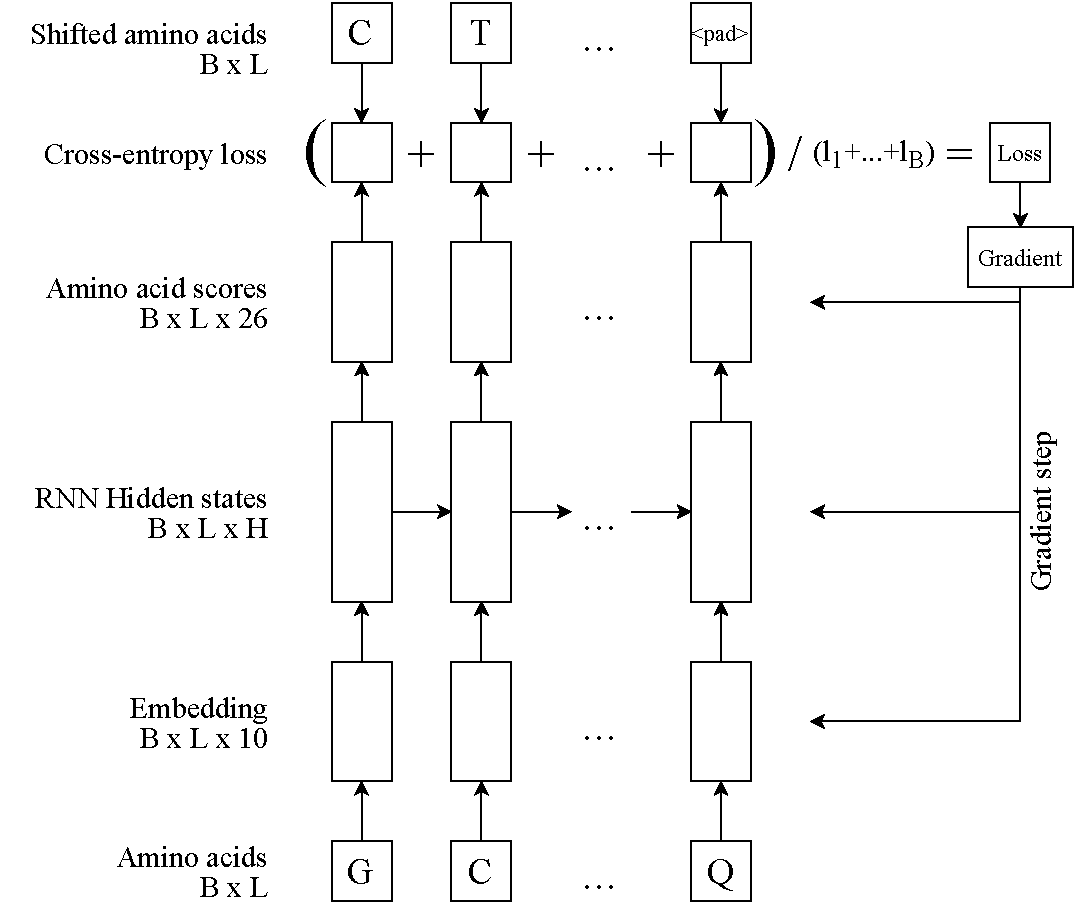
\includegraphics[width = \linewidth]{figures/pretraining_diagram.pdf}
    \caption{Architecture of the model for the unsupervised pretraining. B is batch size, L is the length of the longest protein sequence in the batch, H is the size of the hidden state of the RNN and $\text{l}_n$ is the length of the $n$th protein in the batch. The output size of the linear layer (26) comes from the number of valid amino acids plus some extra utility tokens. Note that the top and bottom layer (the amino acids) in the diagram are equal, except the top is shifted one to the left. Also note that the loss for pad tokens is ignored.}
    \label{fig:pretrain_arch}
\end{figure}

In contrast to the original UniRep, we did not use weight normalization on the RNN, mostly for technical and pragmatic reasons. Using weight normalization in PyTorch at the same time as multi-GPU training (see section \ref{section:pretraining}) turned out to be technically difficult, due to the way PyTorch duplicates the model on each GPU. In addition, weight normalization made the models significantly slower to run, slowing down training.

\subsubsection{Data}
\label{section:reproduction_data}
For data, we downloaded the UniRef50 dataset \cite{uniprot}, the same dataset that the UniRep authors used. From the time between UniRep's training and our reimplementation, the UniRef50 dataset had grown from around 27 million proteins to 39 million proteins. At first, we did not consider this a problem, since we had developed a streaming dataloader which did not need to hold the entire dataset in memory (which would obviously be impossible). However, the dataset's size proved to be a problem for model training -- it could take our largest models more than 12 hours to train a single epoch, during which performance would not increase significantly. Further training proved that the dataset was simply too large for our model to learn from.

Luckily historical versions of UniRef50 are available and, though the UniRep authors did not say exactly which version they used, we managed to find a UniRef50 version (the 2017/11 version) of a similar size, and we assume this is the dataset they used. Still, 27 million proteins was too much for us to handle, so we sampled 102400 proteins for training and 10240 proteins for validation, uniformly at random from this version of UniRef50 (with no overlap on training and validation, of course).

\subsubsection{Hyper-parameter search}\label{reproduction_parameters}
\label{section:hyperparam}
We considered three main hyperparameters for our experiments: the type of recurrent neural network (LSTM, mLSTM and GRU), the dimensionality of the RNNs hidden state (128, 512 and 1024) as well as whether or not to use truncated backpropogation (if yes, with a window of size 256). This gives us 18 different configurations for our model. For convenience, we give each configuration a shorthand name consisting of the RNN used, the hidden state size and a ``T'' if truncated back-propogation was used. For example ``LSTM512T'' is the configuration using an LSTM of size 512 with truncated back-propogation.

\subsubsection{Pretraining}\label{reproduction_pretraining}
\label{section:pretraining}
As mentioned, we trained with 102400 proteins for training, and another separate set of 10240 proteins for validation. We trained each model until the validation loss did not improve, with a patience of 20 epochs. We used a batch size of 1024 for the models using truncated backpropogation and a batch size of 256 for those that did not (for memory reasons). 

% In order to try to combat the lack of training performance of our models, we tried using truncated backpropogation, just as they do in the UniRep paper. This helped our model learn slightly faster, since more gradient updates were made for each protein sequence. Also, the training got simpler, because the gradient only takes into account the operations of the RNN that happened in the truncation window.

% Despite truncated backpropogation, our model still did not improve significantly while training, or at least improved too slowly. We're not sure why the model was reluctant to learn -- perhaps we just simply did not have enough time to train or maybe the model's dimensions were too small for it to learn effectively. We bit the bullet and reduced the size of the training dataset from all the 39 million proteins to a more manageable 102400. Finally we could complete multiple epochs of training within a reasonable time-frame, leading to improved training loss. Especially the LSTM model was capable of achieving a better training loss on predicting the next amino acid than the other two RNNs.

In order to speed up training, we spent some time adapting our model to distributed multi-GPU training. Thankfully, this is not too difficult using PyTorch's \texttt{DataParallel} module\footnote{See \url{https://pytorch.org/docs/stable/nn.html\#torch.nn.DataParallel} for details.}. This allowed us to train on multiple GPUs in parallel. The pretraining was done on 4 Nvidia Titan X GPUs in parallel for all the models.

Most of the models reached their peak validation performance in less than 20 epochs, though a few required a lot more epochs (notably, the GRU128T model required more than 200 epochs of very, very slight improvements before encountering 20 epochs in a row with no performance gain). Most models did not stray very far from the initial validation loss from the first epoch -- a typical improvement over the entire training was from around 3.0 validation loss to somewhere around 2.8 validation loss. Figure \ref{fig:lstm_train_performance} and \ref{fig:gru_train_performance} show the training and validation losses of the LSTM1024T and GRU1024T models respectively, for each epoch of training.

\begin{minipage}{\linewidth}
	\centering
	\begin{minipage}{0.48\linewidth}
		\begin{figure}[H]
			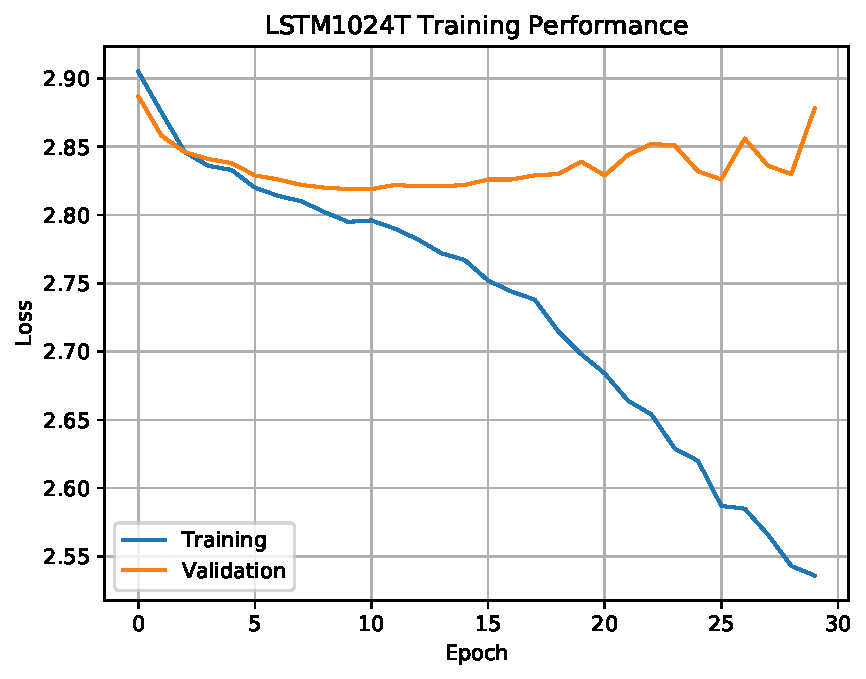
\includegraphics[width=\linewidth]{figures/LSTM1024T_Training_Performance.pdf}
			\caption{Training and validation loss of LSTM1024T.}
			\label{fig:lstm_train_performance}
		\end{figure}
	\end{minipage}
	\hfill
	\begin{minipage}{0.48\linewidth}
		\begin{figure}[H]
			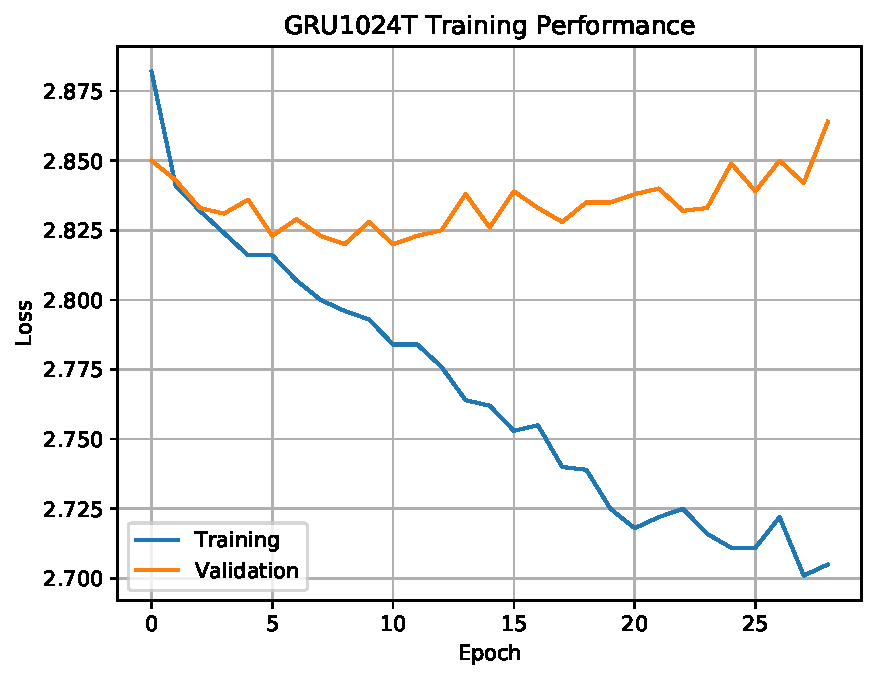
\includegraphics[width=\linewidth]{figures/GRU1024T_Training_Performance.pdf}
			\caption{Training and validation loss of GRU1024T.}
			\label{fig:gru_train_performance}
		\end{figure}
	\end{minipage}
\end{minipage}

\subsubsection{Fine-tuning to TAPE tasks}
We loaded the pretrained models into the TAPE tasks, and trained on each task, until no improvement in the validation loss occurred, with a patience of 20 epochs. The training on the TAPE tasks was done on a single Nvidia Titan X GPU for all the models, with a batch size of 128. Then each model was evaluated on the test split of the TAPE dataset for that task (``ts115'' split for secondary structure, ``test\_fold\_holdout'' for remote homology and simply ``test'' for stability and fluorescence).

\subsection{Results}
\label{section:reproduction_results}
The original UniRep paper makes various inquiries into the produced representations in order to determine its quality. Three of them are (1) how well did the model learn to embed the amino acids, (2) how well does the representations discern proteomes and (3) how well are protein representations separated in terms of their structural classification (SCOP). These correspond to Fig. 2a-c in the UniRep paper \cite{alley2019unified}. We have reproduced variants of these three figures using our implementation, see section \ref{section:amino}, \ref{section:proteome} and \ref{section:SCOPe}. These figures mainly informs the determination of what the underlying representation has learned to retain, and how it relates to different protein properties.

In addition, we have used the produced protein representations on the TAPE tasks in order to evaluate their usefulness in practical settings. These results are described in section \ref{section:TAPE_results}.

\subsubsection{Amino Acid Embeddings}
\label{section:amino}
In order to assess the representations, the model embeddings of the 20 amino acids (O, U excluded) is cast into three dimensions by a principal component analysis for inspection. The resulting points are shown in figures \ref{fig:fig2a_LSTM} and \ref{fig:fig2a_GRU}. There is a tendency of groups with similar properties to be clustered together, but it is not striking. It does suggest that the embeddings capture some of the similarity between amino acids, but enough to clearly capture the variance between them.

\begin{figure}[H]
    \centering
    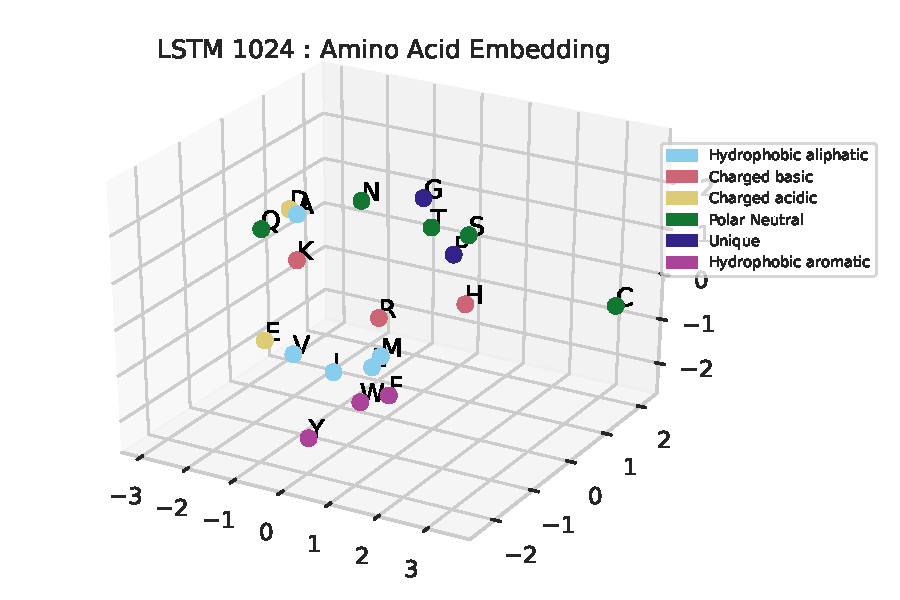
\includegraphics[width=\linewidth]{figures/fig2a_LSTM_1024_no_trunc.pdf}
    \caption{The three most principal components of the amino acid embeddings produced by the LSTM1024 model.}
    \label{fig:fig2a_LSTM}
\end{figure}

\begin{figure}[H]
    \centering
    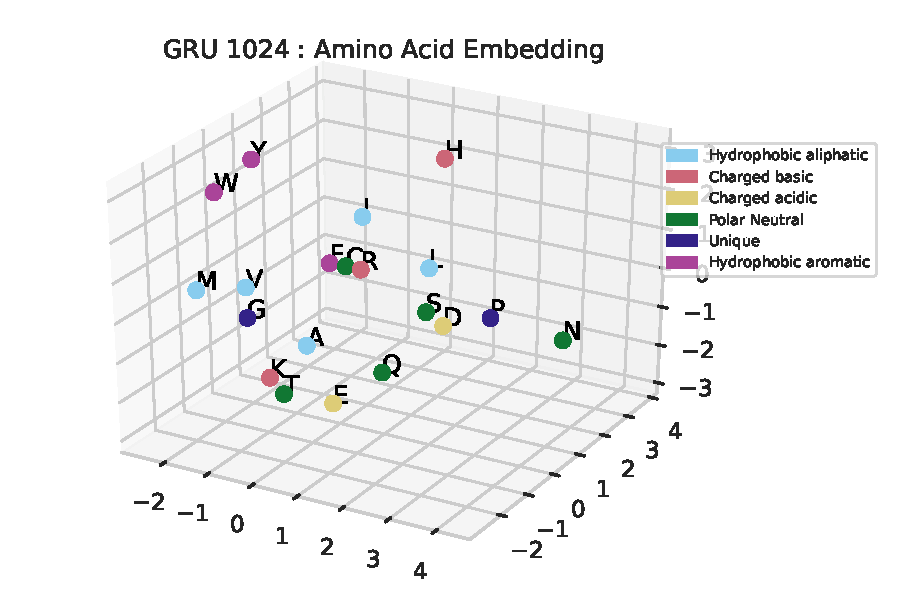
\includegraphics[width=\linewidth]{figures/fig2a_GRU_1024_no_trunc.pdf}
    \caption{The three most principal components of the amino acid embeddings produced by the GRU1024 model.}
    \label{fig:fig2a_GRU}
\end{figure}

The amino acid embedding produced by the full UniRep model seem to clearly separate the hydrophobic amino acids, while the remaining is less separated. Our LSTM-based reimplementation yield a similar result, but otherwise the reproduced amino acid embeddings seem to degrade, presumably due to some of our constraints (time, data size, model architecture). \todo{include mLSTM?}

\subsubsection{Proteome Representations}
\label{section:proteome}
In order to assert representation similarities across organisms, the UniRep authors compare proteome representations produced by the model \cite{alley2019unified}. In this section, we reproduce similar plots, varying the network architecture. The models used are both of 1024 hidden sized and one layered with no truncation, but vary in the neural network, one being GRU-based and one being LSTM \todo{mLSTM also?}. A single proteome consists of a set $P$ of associated proteins. A representation $\ve{r}_p$ of each protein $p$ is produced using the model, and the average of these representations is the final representation $\ve{r}_P$ for the proteome:
\[ \ve{r}_P = \frac{1}{|P|} \sum_{p \in P} \ve{r}_p. \]
In addition, each proteome is classified according to its taxonomic group. This distinction allows us to qualitatively inspect and judge the representations checking if proteome groups are clustered together. The resulting plots can be seen in figure \ref{fig:fig2b_LSTM} and \ref{fig:fig2b_GRU} for LSTM and GRU-based representations, respectively.

\begin{figure}[H]
    \centering
    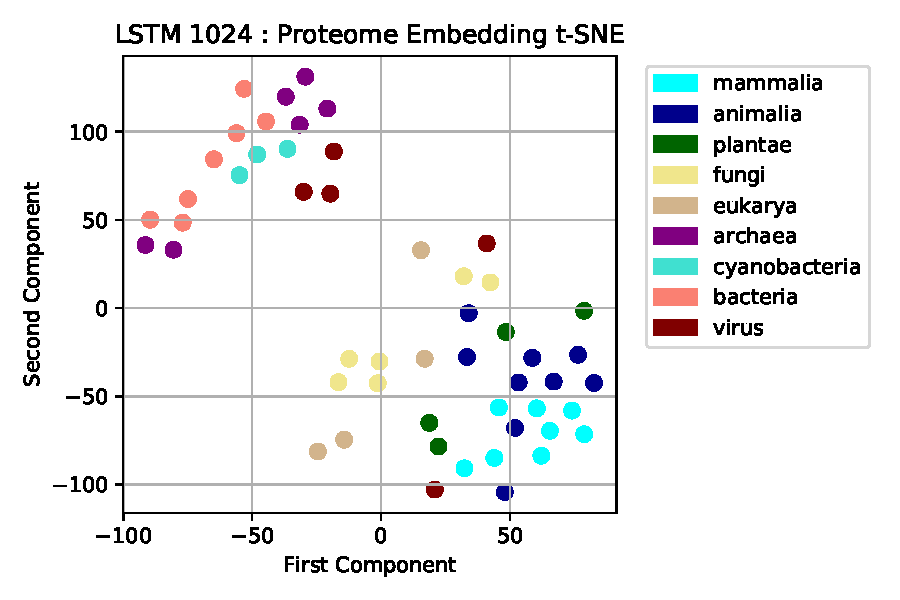
\includegraphics[width=0.95\linewidth]{figures/fig2b_LSTM_1024_no_trunc.pdf}
    \caption{Representations of 9 proteome domains, separated by color. The representations are modeled with a LSTM network of 1024 hidden size. The embeddings are projected onto the plane using t-SNE with perplexity 12.}
    \label{fig:fig2b_LSTM}
\end{figure}

\begin{figure}[H]
    \centering
    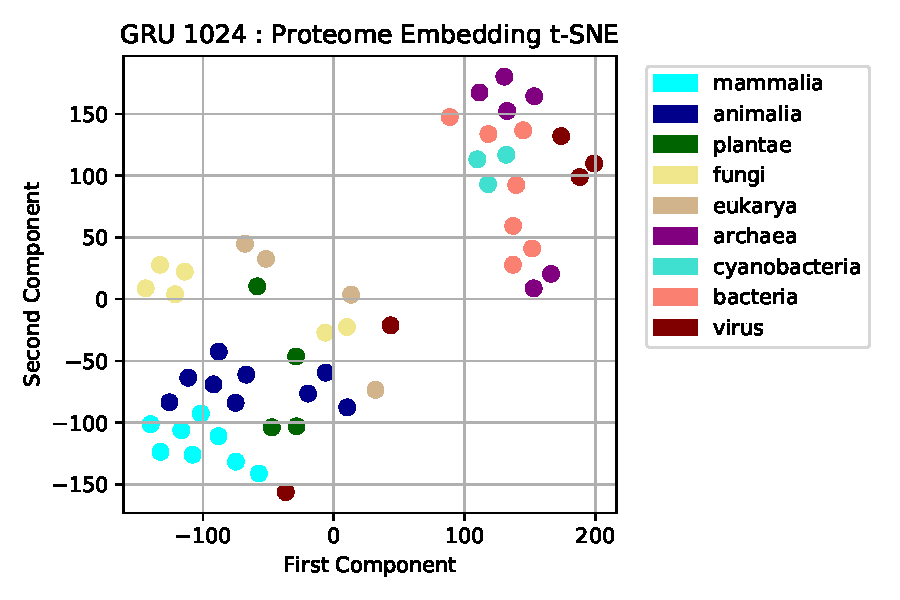
\includegraphics[width=0.95\linewidth]{figures/fig2b_GRU_1024_no_trunc.pdf}
    \caption{Representations of 9 proteome domains, separated by color. The representations are modeled with a GRU network of 1024 hidden size. The embeddings are projected onto the plane using t-SNE with perplexity 12.}
    \label{fig:fig2b_GRU}
\end{figure}

Both (\todo{three? mLSTM}) figures show that the models are capable of making representations that cluster groups together. There are two major clusters: Mammals, animalia, plantae, eukarya and fungi are clustered together, separate from bacteria, virus, cyanobacteria and archaea. This separation is expected as it denotes the eukaryote and procaryote organisms. These figures are very similar to the results in the UniRep paper, indicating that the representations are sufficiently informed to do this well. Another explanation could be that the proteins within a proteome are sufficiently similar that their mean representations simply end up close to each other, regardless of the learned model. The representation is important, but there might be a tendency to see such grouping by the proteomes' proteins inherent similarity alone.

\subsubsection{SCOPe Secondary Structure Representations}
\label{section:SCOPe}
These results inspect the representations ability to separate proteins by their SCOPe classes (alphas, betas, small, etc.). A low dimensional t-SNE tranformation is applied to the protein representations to cast them into two dimensions. Then, a kernel density estimation is made over all proteins of a single class and shown with a contour plot. The results can be seen in figures \ref{fig:fig2c_LSTM} and \ref{fig:fig2c_GRU}.
\begin{figure}[H]
    \centering
    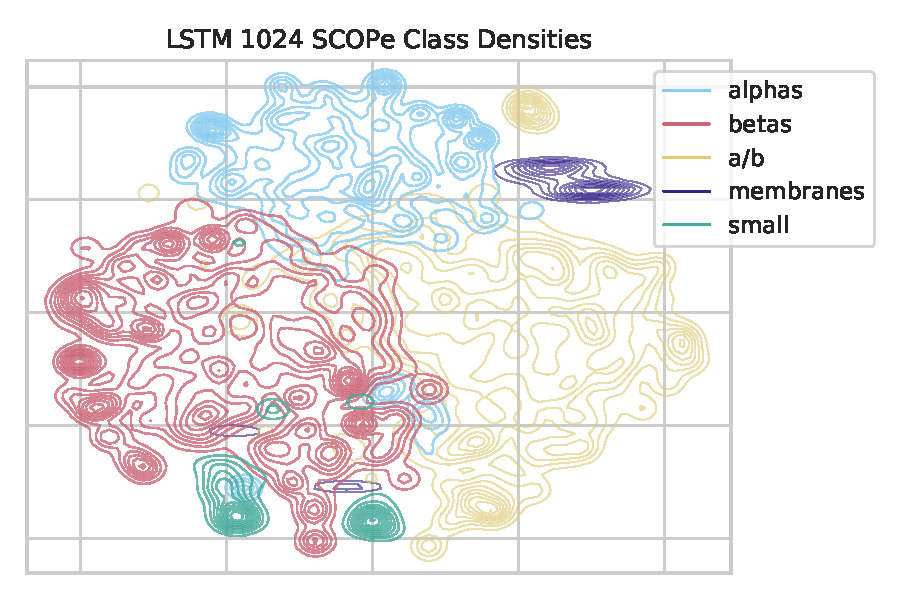
\includegraphics[width=\linewidth]{figures/fig2c_LSTM_1024_no_trunc.pdf}
    \caption{SCOPe class contours made from LSTM-based protein representations cast to two dimensions using t-SNE.}
    \label{fig:fig2c_LSTM}
\end{figure}
\begin{figure}[H]
    \centering
    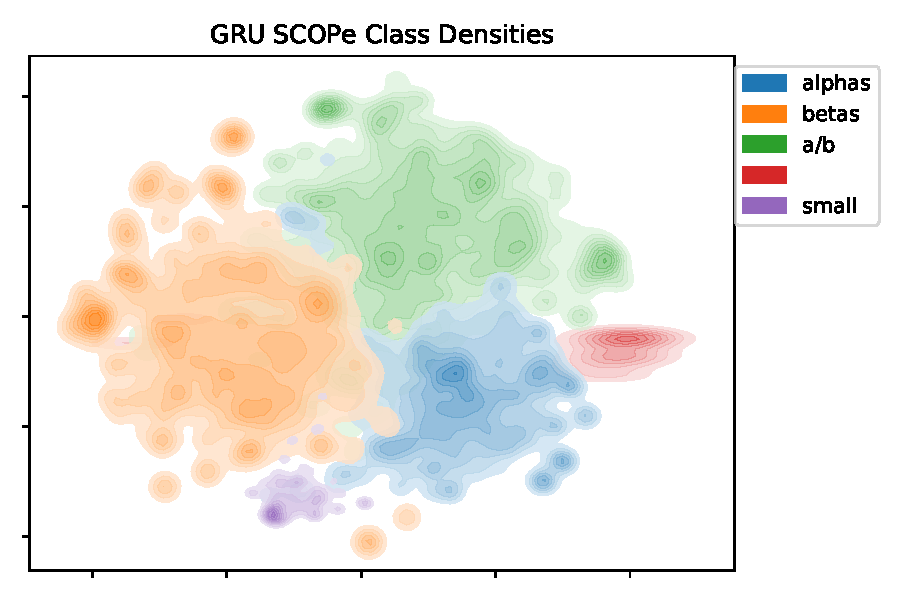
\includegraphics[width=\linewidth]{figures/fig2c_GRU_1024_no_trunc.pdf}
    \caption{SCOPe class contours made from GRU-based protein representations cast to two dimensions using t-SNE.}
    \label{fig:fig2c_GRU}
\end{figure}

\todo{PCA plots}

\todo{mLSTM plots}

\subsubsection{TAPE Tasks}
\label{section:TAPE_results}
In addition to the above figures, we also produced numerical results, by running our models on 4 out of the 5 TAPE tasks, described earlier in \ref{section:tape}. The results can be seen in table \ref{table:taperesults}.

% Exact performance for below 0.6915903582009157
We also tried running a single model (the 1024-size LSTM) on the secondary structure task without pretraining. This model achieved a performance of 0.692, which is quite close to the results displayed in table \ref{table:taperesults}. This suggests that TAPE's training on a specific task is sufficient to achieve good results. Pretraining is thus not crucial for the performance of the models, though it does improve the model slightly.

We did not achieve results for the contact prediction task, due to memory constraints. As far as we understand, training on contact prediction involves a square memory cost, due to each amino acids having to be compared to each other amino acid. This is simply too much for the amount of GPU memory we have available.

\begin{table}[ht]
\ra{1.4}
\begin{tabularx}{\linewidth}{Llllllll}
\toprule
\textbf{Name} & \textbf{RNN} & \textbf{Size} & \textbf{TBP?} & \textbf{Sec. Str.} & \textbf{R. Homology} & \textbf{Fluor.} & \textbf{Stab.} \\ \hline
UniRep     & mLSTM & 1900 & Yes  & 0.73   & 0.23  & 0.67  & 0.73  \\
LSTM1024   & LSTM  & 1024 & No   & 0.718  & 0.125 & 0.679 & 0.676 \\
mLSTM1024  & mLSTM & 1024 & No   &        &       &       &       \\
GRU1024    & GRU   & 1024 & No   & 0.703  & 0.148 & 0.675 & 0.736 \\
LSTM512    & LSTM  & 512  & No   & 0.711  & 0.153 & 0.675 & 0.703 \\
mLSTM512   & mLSTM & 512  & No   &        &       &       &       \\
GRU512     & GRU   & 512  & No   & 0.709  & 0.128 & 0.672 & 0.708 \\
LSTM128    & LSTM  & 128  & No   & 0.714  & 0.114 & 0.668 & 0.744 \\
mLSTM128   & mLSTM & 128  & No   &        &       &       &       \\
GRU128     & GRU   & 128  & No   & 0.704  & 0.124 & 0.671 & 0.696 \\
LSTM1024T  & LSTM  & 1024 & Yes  & 0.700  & 0.123 & 0.676 & 0.783 \\
mLSTM1024T & mLSTM & 1024 & Yes  &        &       &       &       \\
GRU1024T   & GRU   & 1024 & Yes  & 0.693  & 0.103 & 0.676 & 0.746 \\
LSTM512T   & LSTM  & 512  & Yes  & 0.706  & 0.079 & 0.675 & 0.760 \\
mLSTM512T  & mLSTM & 512  & Yes  &        &       &       &       \\
GRU512T    & GRU   & 512  & Yes  & 0.688  & 0.110 & 0.671 & 0.713 \\
LSTM128T   & LSTM  & 128  & Yes  & 0.700  & 0.084 & 0.663 & 0.656 \\
mLSTM128T  & mLSTM & 128  & Yes  &        &       &       &       \\
GRU128T    & GRU   & 128  & Yes  & 0.700  & 0.109 & 0.662 & 0.712 \\ \bottomrule
\end{tabularx}
\caption{Results for 4 of the 5 TAPE tasks. For convenience, each model was given a short-hand name. The table indicates the type of RNN used and the size of the RNN's hidden state. It also indicates whether or not truncated back-propogation (TBP) was used during pretraining. The metric for secondary structure and remote homology is accuracy; for fluorescence and stability it is Spearman's $\rho$. In either case, higher is better. The results for the UniRep model was taken from \url{https://github.com/songlab-cal/tape} -- we did not run the UniRep model ourselves.}
\label{table:taperesults}
\end{table}

\subsection{Discussion}
\label{section:reproduction_challenges}
During our efforts to reimplement the UniRep model, we ran into multiple challenges.

The implementation of the custom mLSTM presented both a theoretical and technical challenge. Firstly, we had to understand the theory behind the mLSTM and the operations it performed. Secondly, we had to actually implement the mLSTM in a PyTorch-compliant manner. This was not trivial, and the resulting RNN was significantly slower and more memory-hungry than a regular LSTM. Still, we opted not to use the JIT capabilities of PyTorch since the speedup was not significant and the errors were harder to debug.

We note that it is much easier to work with existing implementations of neural network layers (like the LSTM and GRU RNNs) in established frameworks like PyTorch, rather than implement custom, novel layers. This ease of use and experimentation might have an influence on which models are explored, and which are not -- for example, in this work we only considered one custom RNN, despite a huge number of variants on LSTMs existing. The implementation of ``non-standard'' layers (like the mLSTM) in major frameworks could increase the exposure of other types of models and possibly lead to more varied architecture exploration, ultimately leading to better models.

The size of the largest models (especially mLSTM1024) presented a practical challenge, in that training and using such huge models is slow and often full of memory allocation errors. The hardware requirements for such models also make them difficult to reproduce -- for instance, we did not even attempt to reproduce the 1900 RNN hidden state size that the UniRep authors used. We were fortunate enough to be granted access to our institute's compute cluster. This reimplementation project would have been entirely impossible without the hardware provided by this cluster.

As it turns out, making huge models seems not to be entirely necessary anyway. As table \ref{table:taperesults} shows, similar performance can also be obtained by much smaller models. While large models perform marginally better, smaller models are superior in other ways. First and foremost, the requirements to actually use such a model is severely reduced, making the model useful to more people. It is also much faster to train.

There are also costs associated with larger models. There is a financial cost; large models require fast, expensive hardware, which may not be readily available to individuals, small businesses or even poorly funded research institutions. There is also an environmental cost. Recent literature within the NLP field has voiced concerns about the environmental damage that huge deep learning models may cause \cite{strubell2019energy}. In \cite{greenai}, Schwartz, Dodge et al. discuss ways to evaluate models by cost-efficiency in addition to usual metrics like accuracy.

The UniRep article is not innocent in this aspect -- after all, they trained on 4 Nvidia K80 GPUs for 3.5 weeks. Not only do K80 GPUs go for more than 3,000£ ($\approx$ 4000 USD or 25000 DKK) on Amazon, at the time of writing, but running them for weeks is not without costs either. Some quick back-of-the-envelope calculations suggests that the electricity used in training UniRep has resulted in emissions equivalent to over 150 kg CO2\footnote{The power limit of the K80 is 300W (see \url{nvidia.com/content/dam/en-zz/Solutions/Data-Center/tesla-product-literature/Tesla-K80-BoardSpec-07317-001-v05.pdf} for details). Assume 50\% usage. $4 \cdot 150\text{W} \cdot 50\% \cdot 3.5\text{weeks} \approx 350\text{kWh}$. Assume 0.4483 kg of CO2 per kWh (see \url{epa.gov/energy/emissions-generation-resource-integrated-database-egrid} for details). $350\text{kWh} \cdot 0.4483 \frac{\text{kg CO2}}{\text{kWh}} \approx 150 \text{kg CO2}$}. This is more CO2 than that emitted by an entire loaded airliner flying from Copenhagen to London\footnote{\url{travelnav.com/emissions-from-copenhagen-denmark-to-london-united-kingdom}}. Of course, our models are not innocent in this regard either, though we haven't trained for nearly as much time, per model or in total.

Even the amount of data used in the UniRep article seems excessive. We achieved similar results by sampling less than 0.5\% of the training data. More data is of course not a bad thing, but this also makes the model more difficult and costly to train. When considering 22 million data points, perhaps one should wonder when to stop.

\clearpage
\section{Conclusion}
In section \ref{section:unirep_reproduction} we have presented the main new work of this project: the architectural reimplementation of the UniRep protein representation model and a subset of core results from the UniRep article \cite{alley2019unified}. In section \ref{section:reproduction_results} we show that it is possible to achieve protein representations that are produced by down-scaled models that yield comparable performance with the full UniRep model. The model learns to construct meaningful amino acid embeddings as seen in \ref{fig:fig2a_LSTM}. Our representations manage to retain information what is sufficiently general across proteins to cluster proteomes and secondary structure, comparable to the UniRep full model (figures \ref{fig:fig2b_LSTM} and \ref{fig:fig2c_LSTM}). These results indicate that the reproduced model is sufficiently capturing the behavior of the UniRep model. 

In section \ref{section:TAPE_results} an ablation study of various model instances show that it is possible to achieve performance on downstream tasks with several alternative model designs. Size variation show that larger models yield marginally better performance, at the cost of computations and hardware requirements.

The reimplementation process also gave rise to some practical complications: In section \ref{section:reproduction_challenges} we enumerate major challenges and discuss the consequences. Scaling data and neural networks in size cause practical issues that do not extend to smaller models, namely how to efficiently train and compute model parameters. We found that such practicalities cause a significant barrier to what can be sufficiently reimplemented within the time and specification of a project such as ours.

In section \ref{section:unirep_discussion}, we discussed the design choices of the model. Specifically, we discussed the choice of making a representation of a protein sequence that is constituted by the average of the hidden states at each position in the sequences. This choice does not preserve any position-related features of the protein, nor does it easily allow for a reversible procedure, regaining the sequence from its representation. Finally, it complicates the interpretation of the representation: units that give a clear signal to some property of the protein in local positions potentially loose relevancy when averaged. These arguments suggest that even though the representation capture fundamental protein features that performs well in downstream tasks, the design of the representation is problematic for other tasks, e.g. tasks that require a feature space where the representation can be reversed.

% project description
% In this work, we wish to reproduce the results of the aforementioned authors, as well as review and critique the methods and design choices they made. We will attempt to evaluate in which aspects their model is strong, and in what aspects it is weak. In addition, we will reflect on alternative approaches, in order to find new ways of tackling the problem. In doing so, we will learn more about (unsupervised) representation learning and protein informatics.


% train discussion points
% - language modelling validation: does it learn? very low accuracies after ~10 epochs
% - no truncation is (it seems) better than truncation. this makes sense as doing gradient on entire sequence is more informative than doing it on truncated subsequences, and thus leads to better parameters
% training on 102400 data points instead of millions

\clearpage
\section{Further work}
The field of protein deep learning has seen great recent developments, including the above-mentioned UniRep model. These advances suggests that there is potential within the field and much more still to be explored.

As we discussed in section \ref{section:unirep_discussion}, there are many things that could be reconsidered about the UniRep model's architecture. Indeed, if we again consider the breadth of methods used in natural language processing, there are several methods that have yet to be explored in the protein deep learning scene.

One key advantage of UniRep is its ability to encode a protein into a point in a high-dimensional latent space. However, one key disadvantage is that this point cannot be \textit{decoded} back into a protein sequence. Such decoding could be very useful, if one wanted to explore the latent space for candidate desirable proteins. One aspect that we would like to explore further in the future is a model's ability to decode its representation back to a protein.

One way of achieving this ability is using an encoder-decoder architecture, which is a very common technique within natural language processing. Using an encoder-decoder architecture in an unsupervised manner results in what is known as an \textit{auto-encoder}. Auto-encoders inherently have the ability to both encode and decode, and could possibly be a very useful architecture for protein deep learning. There are also interesting variants of auto-encoders such as the variational auto-encoder which, in addition to encoding and decoding, provides a probability distribution over the representations.

We would also like to explore the possibility of making representations of more localized families of proteins. Making meaningful representations over the entire space of all proteins is, honestly, very optimistic. The similar task within natural language processing is reasonable, but consider also that the number of words in all the languages of the world is effectively zero in comparison to the number of possible protein sequences. Specializing models to specific protein families (like NLP models specialize to languages) may be a way to reduce the complexity of the problem and achieve better performance. Such models may also be smaller than models attempting to represent the entire protein space, and may thus be both financially and environmentally superior.

It is clear that there are plenty of avenues for further work in protein deep learning and we look forward to what the future of the field may bring.

% \section*{UniRep}
% The UniRep model \cite{alley2019unified} enables stability prediction of proteins, and so one claim is that this allows for the UniRep model by work as a basis for the prediction of protein function directly from protein sequence (ref).

% References
\clearpage
\addcontentsline{toc}{section}{References}
\printbibliography[title={References}]

\end{document}
